%%%%%%%%%%%%%%%%%%%%%%%%%%%%%%%%%%%%%%%%%%%%%%%%%%%%%%%%%%%%%%%%%%%%%%
% Problem statement
\begin{statement}[
  problempoints=110,
  timelimit=1 second,
  memorylimit=512 MiB,
]{Lampice}

\setlength\intextsep{-0.1cm}
\begin{wrapfigure}[7]{r}{0.2\textwidth}
\centering
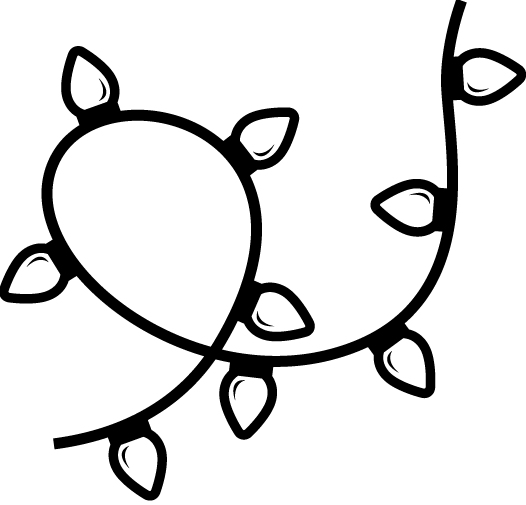
\includegraphics[width=0.2\textwidth]{img/lampice.png}
\end{wrapfigure}

Mirko chose a Christmas tree for the upcoming holidays and decided to decorate
it with Christmas lights. Christmas lights contain $N$ LED lights that are
connected via $(N-1)$ conductive wires such that all of the lights are connected.
Additionally, we know the color of each Christmas light.

After he decorated the tree, Mirko proudly stared at his masterpiece. After a
while, he started noticing different patterns. Among those patterns, he was
particularly amazed by so-called \textit{palindromic segments}. Palindromic
segment is a segment of Christmas lights on the path between two fixed lights,
$u$ and $v$, such that the array of colors on a path from $u$ to $v$ is exactly
the same as the array of colors on the path from $v$ to $u$.
Determine the length of the longest palindromic segment
expressed in the number of lights on that segment.

%Mirko wants to find the longest palindromic segments, but there are too many
%lights! Help him, and determine the length of the longest palindromic segment
%expressed in the number of lights on that segment.

%%%%%%%%%%%%%%%%%%%%%%%%%%%%%%%%%%%%%%%%%%%%%%%%%%%%%%%%%%%%%%%%%%%%%%
% Input
\subsection*{Input}
The first line contains an integer $N$ $(1 \le N \le 50\ 000)$ from the task
description.

The next line contains an array of $N$ lowercase letters from the English
alphabet where the $i$-th letter represents the color of the $i$-th Christmas
light.

Each of the next $(N - 1)$ lines contains two integers $A$ and $B$
$(1 \le A, B \le N, A \neq B)$, which denote that lights $A$ and $B$
are directly connected by a conducting wire.

%%%%%%%%%%%%%%%%%%%%%%%%%%%%%%%%%%%%%%%%%%%%%%%%%%%%%%%%%%%%%%%%%%%%%%
% Output
\subsection*{Output}
The first line of output should contain the length of the longest
palindromic segment.

%%%%%%%%%%%%%%%%%%%%%%%%%%%%%%%%%%%%%%%%%%%%%%%%%%%%%%%%%%%%%%%%%%%%%%
% Scoring
 \subsection*{Scoring}
{\renewcommand{\arraystretch}{1.4}
  \setlength{\tabcolsep}{6pt}
  \begin{tabular}{ccl}
 Subtask & Score & Constraints \\ \midrule
  1 & 17 & $N \le 3000$ \\
  2 & 25 & \makecell[l]{
            % božićne lampice čine lanac, tj.
            Light $i$ is directly connected with light
            $i+1$ $(1 \le i < N)$.
            } \\
  3 & 31 & At most $100$ lights are directly connected with exactly one other light. \\
  4 & 37 & No additional constraints. \\
\end{tabular}}

%%%%%%%%%%%%%%%%%%%%%%%%%%%%%%%%%%%%%%%%%%%%%%%%%%%%%%%%%%%%%%%%%%%%%%
% Examples
\subsection*{Examples}
\begin{tabularx}{\textwidth}{X'X'X}
\sampleinputs{test/lampice.dummy.in.1}{test/lampice.dummy.out.1} &
\sampleinputs{test/lampice.dummy.in.2}{test/lampice.dummy.out.2} &
\sampleinputs{test/lampice.dummy.in.3}{test/lampice.dummy.out.3}
\end{tabularx}

%%%%%%%%%%%%%%%%%%%%%%%%%%%%%%%%%%%%%%%%%%%%%%%%%%%%%%%%%%%%%%%%%%%%%%
% We're done
\end{statement}

%%% Local Variables:
%%% mode: latex
%%% mode: flyspell
%%% ispell-local-dictionary: "croatian"
%%% TeX-master: "../hio.tex"
%%% End:
